\documentclass[11pt,a4paper]{article}
\usepackage{tikz}
\usetikzlibrary{arrows.meta,positioning}
\usepackage{tabularx}
\usepackage{amsmath,amssymb,amsthm}
\usepackage{geometry}
\geometry{margin=1in}
\usepackage{hyperref}
\usepackage{graphicx}
\usepackage{setspace}
\onehalfspacing

\title{\textbf{Paper B-01: Unified Infrastructure:\\ A Constraint-Driven Flux Dynamics (CDFD) Perspective}}
\author{Steve Bico Mujjabi, MD\\
\small Independent Researcher\\
\small Founder, Vura Labs\\
\small Kampala, Uganda\\
\small ORCID: 0009-0001-0556-5516}
\date{August 2026}

\begin{document}
\maketitle

% BEGIN SHARED-METHODS POINTER
\noindent\textit{Shared Part IV notation and evidence boundaries are defined in \path{PART_IV_METHODS_AND_CLAIM_BOUNDARY.md}. This paper states only its local observables, comparison, and failure conditions.}
% END SHARED-METHODS POINTER


\begin{abstract}
This paper develops a falsifiable CDFD/AFL model of Unified Infrastructure. It maps demand across energy, water, transport, communication, and public services to driving flux $\Phi$, component capacity, coupling, dependency, and maintenance limits to active constraint $C$, redundancy, rerouting, control, repair, and demand management to responsiveness $S$, and aging, backlog, design choices, and prior incidents to structural memory $M_s$. The target outcome is service continuity, cascade size, restoration, and equity, tested against sensor streams, service logs, asset registers, dependency maps, and incident records. The paper treats universality as a shared model architecture rather than an assertion that unlike systems have the same material mechanism. It states the negative result that would make the mapping unnecessary and places the domain claim inside the cumulative CDFD programme and its reproducible runtime boundary.
\end{abstract}

\section{Introduction}

A modern city is a stack of overlapping transport networks. A failure in the electrical grid instantly impacts the water pumping stations; a flooded highway halts the delivery of fuel to backup generators. These networks are not isolated; they are thermodynamically coupled.

CDFD provides a common audit language for this coupling. Traffic, packet routing, and blood flow have different governing mechanisms, but each can be tested for measurable bottlenecks, network dependence, overload, and recovery.

\section{The Meta-Infrastructural Adaptive Surface}
We govern the unified infrastructure using the Adaptive Operating Ratio:
\begin{equation}
    \Psi_s = \left( \frac{\Phi}{C} \right) \cdot S \cdot M_s
\end{equation}

For a unified urban grid:
\begin{itemize}
    \item \textbf{Flux ($\Phi$)}: The aggregate volumetric throughput of all vital resources (power, water, data, logistics).
    \item \textbf{Constraint ($C$)}: The physical limitations of pipes, wires, and roads, as well as the geographical bottlenecks (e.g., a single bridge connecting two landmasses).
    \item \textbf{Responsiveness ($S$)}: Systemic redundancy and the capacity of the infrastructure to dynamically reroute flux through alternative physical mediums.
    \item \textbf{Memory ($M_s$)}: Sunk costs and legacy infrastructure. Aging, centralized power plants and century-old water mains represent highly locked structural memory. They force the topology to remain rigid, incapable of adapting to modern, decentralized flow requirements.
\end{itemize}

\subsection{Cross-Domain Cascading Failure}
Consider a severe weather event (e.g., a hurricane). The external environmental constraint $C$ spikes massively. The electrical grid loses a major substation. Its local adaptive ratio drops to $\Psi_s \ll 1$. The power flux $\Phi_{elec}$ ceases.

Because the water pumping network relies entirely on $\Phi_{elec}$, the cessation of power acts as an infinite constraint $C_{water}$ on the hydrological network. The water flux $\Phi_{water}$ drops to zero. Consequently, hospitals and factories lose their operational responsiveness $S$.

The failure cascades across domains because the infrastructural memory ($M_s$) was designed with linear dependencies rather than highly cross-linked, decentralized redundancy. A truly unified, CDFD-optimized infrastructure would feature distributed micro-grids and localized resource generation (high $S$, low $M_s$), ensuring that a constraint spike in one physical domain does not force the topological collapse of the others.



\section{Measurement Layer}

% BEGIN PART IV MAJOR CROSS-DOMAIN UPGRADE
\section{Cross-Domain Model Upgrade: Mechanism, Scale, and Tests}

\subsection{Observable Translation}

The paper-specific translation begins with an observable chain rather than a
verbal analogy. For Unified Infrastructure, the proposed drive is demand across energy, water, transport, communication, and public services.
The active limitation is component capacity, coupling, dependency, and maintenance limits. Responsiveness is carried by
redundancy, rerouting, control, repair, and demand management, while retained state is represented by
aging, backlog, design choices, and prior incidents. The outcome to explain is service continuity, cascade size, restoration, and equity.

\begin{table}[htbp]
\centering
\small
\caption{Operational CDFD/AFL map for Paper B-01.}
\begin{tabularx}{\textwidth}{|l|X|X|}
\hline
\textbf{Term} & \textbf{Paper-specific observable meaning} & \textbf{Measurement question} \\
\hline
$\Phi$ & demand across energy, water, transport, communication, and public services & What rate, load, gradient, or demand enters the focal system? \\
\hline
$C$ & component capacity, coupling, dependency, and maintenance limits & Which measured bottleneck limits transfer, function, or recovery? \\
\hline
$S$ & redundancy, rerouting, control, repair, and demand management & Which process changes effective capacity or reroutes the load? \\
\hline
$M_s$ & aging, backlog, design choices, and prior incidents & Which retained state makes equal present loads produce different futures? \\
\hline
$Y$ & service continuity, cascade size, restoration, and equity & Which outcome is predicted out of sample, with uncertainty? \\
\hline
\end{tabularx}
\end{table}

\begin{figure}[htbp]
\centering
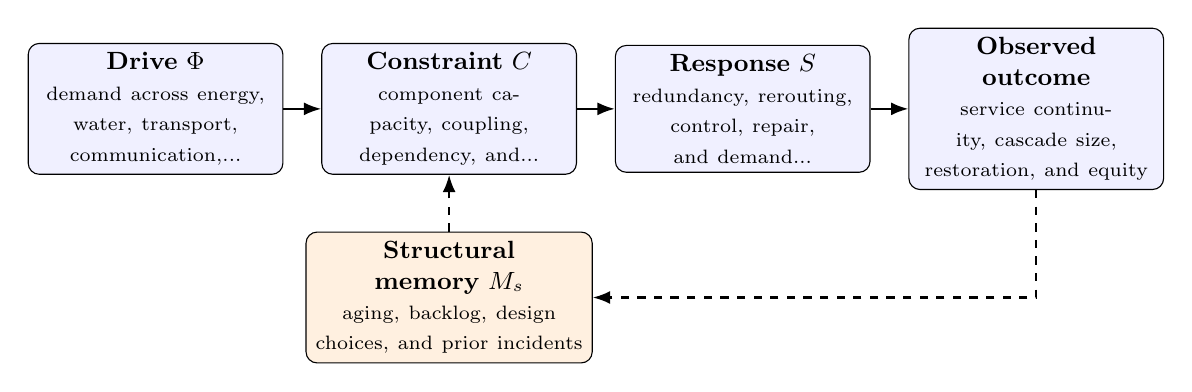
\begin{tikzpicture}[
    node distance=0.48cm,
    every node/.style={font=\small},
    box/.style={draw, rounded corners, align=center, minimum height=1.45cm, text width=3.0cm, fill=blue!6},
    memory/.style={draw, rounded corners, align=center, minimum height=1.25cm, text width=3.4cm, fill=orange!12},
    flow/.style={-{Latex[length=2.2mm]}, thick},
    feedback/.style={-{Latex[length=2.2mm]}, thick, dashed}
]
\node[box] (drive) {\textbf{Drive $\Phi$}\\\scriptsize demand across energy, water, transport, communication,...};
\node[box, right=of drive] (constraint) {\textbf{Constraint $C$}\\\scriptsize component capacity, coupling, dependency, and...};
\node[box, right=of constraint] (response) {\textbf{Response $S$}\\\scriptsize redundancy, rerouting, control, repair, and demand...};
\node[box, right=of response] (outcome) {\textbf{Observed outcome}\\\scriptsize service continuity, cascade size, restoration, and equity};
\node[memory, below=0.72cm of constraint] (memory) {\textbf{Structural memory $M_s$}\\\scriptsize aging, backlog, design choices, and prior incidents};
\draw[flow] (drive) -- (constraint);
\draw[flow] (constraint) -- (response);
\draw[flow] (response) -- (outcome);
\draw[feedback] (outcome.south) |- (memory.east);
\draw[feedback] (memory.north) -- (constraint.south);
\end{tikzpicture}
\caption{Paper B-01 observable CDFD/AFL architecture for Unified Infrastructure. Solid arrows give the proposed forward chain; dashed arrows make history-dependent feedback explicit.}
\label{fig:b01-architecture}
\end{figure}

\subsection{Paper-Specific Causal Hypothesis}

For this paper, the hypothesized causal sequence is specific. A change in
demand across energy, water, transport, communication, and public services arrives faster than redundancy, rerouting, control, repair, and demand management can compensate.
This raises or redistributes component capacity, coupling, dependency, and maintenance limits. If the load persists,
the retained state encoded by aging, backlog, design choices, and prior incidents changes the next response, so a later event of equal
magnitude can produce a different trajectory in service continuity, cascade size, restoration, and equity. The
scientific task is to estimate that sequence against the best ordinary model of
the domain, not merely to redescribe the outcome after it occurs.

\subsection{Cross-Scale Translation Without Mechanistic Erasure}

For the engineered systems family, the cross-domain translation compares demand, designed capacity, feedback control, dependency topology, and accumulated technical state. The strongest engineering use is prospective: the mapping must identify a bottleneck, a control action, or a recovery signature before the failure occurs. \cite{BarabasiAlbert1999,WattsStrogatz1998,Shannon1948,BakTangWiesenfeld1987}
The required scale declaration for this paper is milliseconds to decades; components to national infrastructure. At short
scales, the key question is whether the incoming drive is transmitted,
buffered, or diverted. At intermediate scales, response changes effective
capacity and network exposure. At long scales, retained structure can alter the
state space itself. A result is genuinely cross-scale only when the aggregation
rule is stated and the same conclusion is not an artifact of averaging.

\subsection{Evidence Ladder and Discriminating Tests}

\begin{table}[htbp]
\centering
\small
\caption{Evidence ladder for Paper B-01. Each rung can fail independently.}
\begin{tabularx}{\textwidth}{|p{0.17\textwidth}|X|X|}
\hline
\textbf{Test} & \textbf{Design} & \textbf{Discriminating result} \\
\hline
Proxy audit & Measure sensor streams, service logs, asset registers, dependency maps, and incident records and preregister how each record maps to $\Phi$, $C$, $S$, $M_s$, and $Y$. & The mapping fails if proxies are non-identifiable, circular, or change meaning across cases. \\
\hline
Load ramp & Apply or observe a localized component loss during peak cross-service demand while estimating the dominant constraint and response time. & A threshold claim requires a reproducible nonlinear change and uncertainty bounds, not a visually chosen breakpoint. \\
\hline
Recovery and memory & Match present load across units with different histories, then compare recovery paths. & The memory claim requires history-dependent divergence after current conditions are controlled. \\
\hline
Model comparison & Compare the baseline domain model with and without the CDFD/AFL state variables using held-out data. & The paper's stated falsifier is: coupled CDFD variables do not improve failure or restoration prediction. \\
\hline
\end{tabularx}
\end{table}

\subsection{Research Programme and Boundary Conditions}

The immediate research programme has four steps. First, construct a documented
dataset from sensor streams, service logs, asset registers, dependency maps, and incident records and retain raw units before normalization.
Second, fit a baseline domain model and report its calibration and out-of-sample
error. Third, add the smallest identifiable CDFD/AFL state extension and test
whether it improves prediction of service continuity, cascade size, restoration, and equity. Fourth, repeat the
analysis across the declared scale range and publish negative cases as part of
the cross-domain translation audit.

% END PART IV MAJOR CROSS-DOMAIN UPGRADE

\section{Conclusion}
Engineered infrastructure is a macroscopic organism. Treating power, water, and transit as separate entities defies the basic laws of thermodynamics. By utilizing CDFD, urban planners can design globally coupled, highly elastic infrastructures that natively resist cross-domain cascading failures, ensuring the continuous survival of the metropolitan active surface.
\section*{Conflict of Interest} The author declares no conflict of interest.
\section*{Data Availability}
Part-specific runtime diagnostics are under each Part's \path{outputs/} directory.

Release-wide code: \path{Part_E_Synthesis/supplementary/}.

Generated summaries: \path{Part_E_Synthesis/outputs/}.

Figures: \path{Part_E_Synthesis/figures/}.


\section{Reference Layer}
\bibliographystyle{plain}
\bibliography{universal_afl_references}
\end{document}
